\begin{flushleft}
	
	\titleformat {\chapter} {\normalfont\huge\bfseries\color{black}}   {\thechapter}{10pt}{\huge} 
	\chapter {Data and Class Elements }
	
	\section{Data elements}
	
	\subsection{Entity Relationship Diagram}
	\vspace*{1\baselineskip}
	\begin{figure}[htbp]
		\begin{center}
			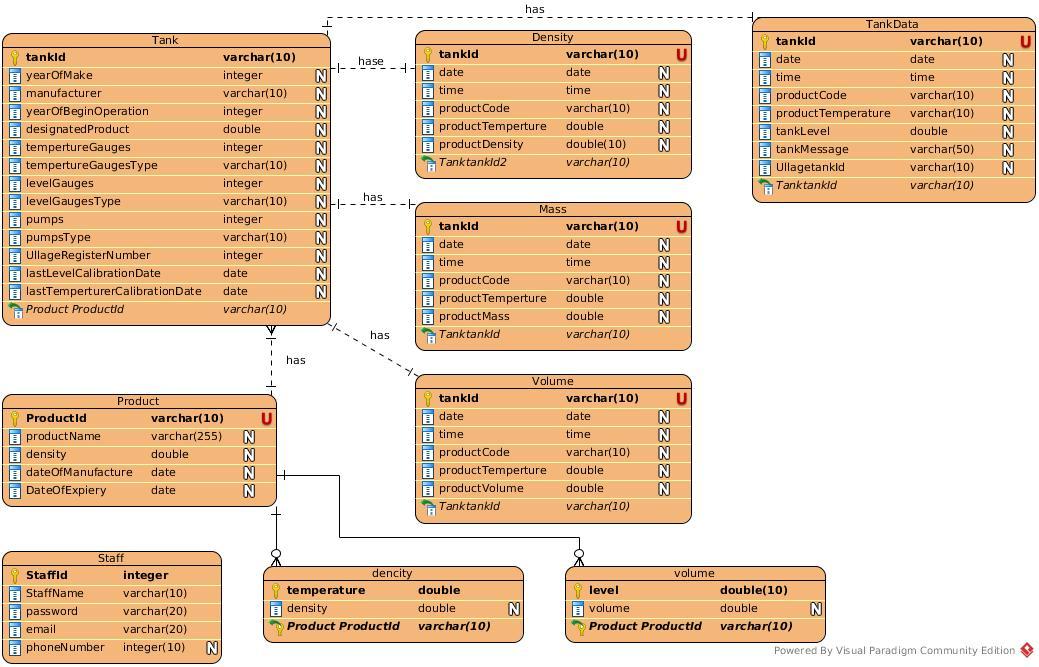
\includegraphics[width=1.00\linewidth]{./images/ERD.jpeg}
			\caption{Entity Relationship Diagram for Tank Farm Inventory System.}
			\label{fig:ERD.jpeg}
		\end{center}
	\end{figure}
	\subsection{Description}
	\vspace*{1\baselineskip}
	\begin{enumerate}
		\item The tanks contain all the details of the tank.
		\item Each tank must has volume.
		\item Each tank must has mass.
		\item Each tank must has tank data.
		\item Each tank must has product details.
		\item Each product must has density details.
		\item Each product must has volume details.
		\item Staff must possess with staff details.
	\end{enumerate}
	
	\newpage	
	\subsection{Class Diagram}
	\vspace*{1\baselineskip}
	\begin{figure}[htbp]
		\begin{center}
			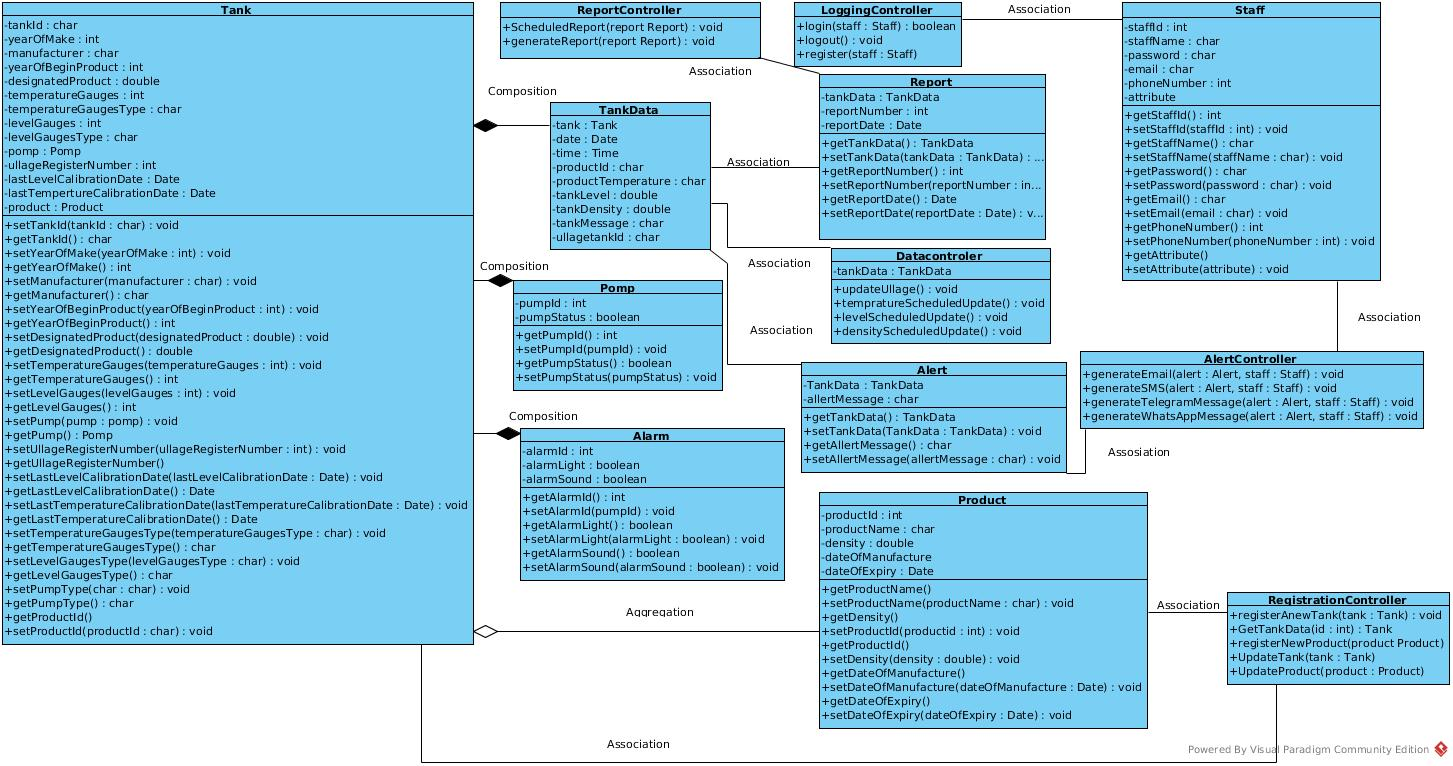
\includegraphics[width=1.00\linewidth]{./images/ClassDiagram.jpg}
			\caption{Class Diagram for Tank Farm Inventory System.}
			\label{fig:ClassDiagram.jpg}
		\end{center}
	\end{figure}
	
	\subsection{Description}
	\vspace*{1\baselineskip}
	\noindent{
		Based on figure 2.2, Subset of the classes in this diagram are the data classes which correspond to entities in the system\\}
	
		\begin{itemize}
			\item Tank : It contains the tank attributes and behaviour.
			\item TankData : It containssome product attributes and behavior which is in the tank.
			\item Pomp : Each tank has pomp and this class consists of pomp attributes and behavior.
			\item Alarm : Each tank has alarm and this class consists of alarm attributes and behavior.
			\item Product : It contains product attributes and behavior.
			\item Staff : It contains staff attributes and behavior.
			\item Report : It contain report attributes and behavior.
			\item Alert : It contains alert attributes and behavior.
		\end{itemize}
		
	\vspace*{1\baselineskip}
	\noindent{
		Subset of the classes in this diagram are the class which control the process flow in the system\\}
	
	\begin{itemize}
		\item Login Controller : It use to do some user process like login,logout and registration.
		\item Report Controller : It use to do some report like generating manual report and scheduled report.
		\item AlertController : It use to do some alert process like login,logout and registration.
		\item RegisterController :  It use to do some product and tank registration and process registration.
		\item DataController : It use to do some update process for both manual and scheduled data.
	\end{itemize}	
    
	
	
\end{flushleft}